\documentclass[a4paper]{article}

\usepackage[utf8]{inputenc}

\usepackage{url}
\usepackage{hyperref}

\usepackage{caption}

\usepackage{listings}

\usepackage{color}

% *** GRAPHICS RELATED PACKAGES ***
%\usepackage[pdftex]{graphicx}
\usepackage{graphicx}
%\usepackage[dvips]{graphicx}
% to place figures on a fixed position
\usepackage{float}

\usepackage[margin=1in]{geometry}

\title{Blockhain Tutorial – syllabus}
\author{}
\date{}


\begin{document}

\maketitle

\tableofcontents

\section{Introduction}

Introduce this tutorial : topics discussed, high-level overviewe of the excersises

\section{Blockchain concepts,basiscs}

desrcibe main concepts of Blockchain 

The introduction to Mininet, OpenFlow and POX controller can be read in the
\href{https://qosip.tmit.bme.hu/foswiki/pub/Meres/OpenFlowMSc/OpenFlow-Mininet-syllabus-en.pdf}{OpenFlow \& Mininet
    syllabus}. On
Figure~\ref{fig:Lab-topo} the network topology used in this P2P lab is shown.

\begin{figure}[H]
    \centering
    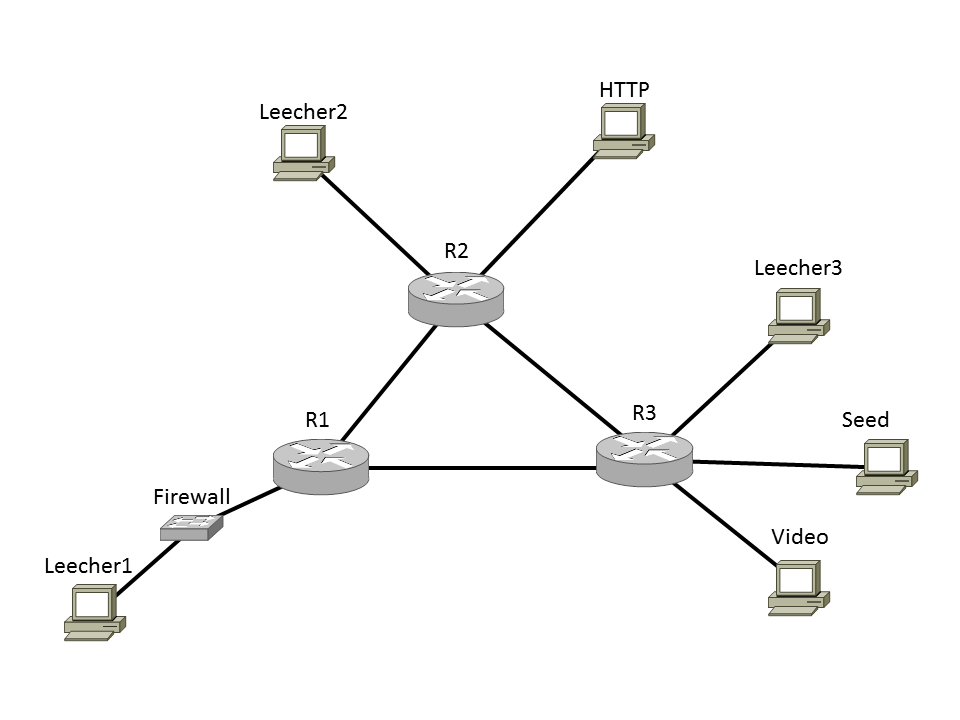
\includegraphics[width=0.9\textwidth]{figures/halozat.png}
    \caption{Network architecture used in lab exercises}
    \label{fig:Lab-topo}
\end{figure}

\begin{lstlisting}[language=python,frame=single,breaklines]
packet = event.parsed  
\end{lstlisting}


\section{Smart contracts}


\section{Smart contracts using Ethereum}


\section{Introduction to the demo environment}

\section{Tutorial exercises}

\subsection{Transaction using the console}
send transaction using console, analyze transaction receipt, analyze blocks, etc.

\subsection{PowerBid game}
Describe game, tasks, evaluation etc.

\subsection{Implement a number guessing game}

\end{document}